% CineLake - Ingestion Layer report
\documentclass[12pt,a4paper]{article}

\usepackage[utf8]{inputenc}
\usepackage[T1]{fontenc}
\usepackage[english]{babel}
\usepackage{lmodern}
\usepackage[margin=2.5cm]{geometry}
\usepackage{booktabs,tabularx,longtable,array}
\usepackage{graphicx}
\usepackage{xcolor}
\usepackage{listings}
\usepackage{tikz}
\usetikzlibrary{positioning,arrows.meta,fit,backgrounds,shapes.geometric,calc}
\usepackage{pgfplots}
\usepgfplotslibrary{groupplots}
\pgfplotsset{compat=1.17}
\usepackage{enumitem}
\usepackage{caption}
\usepackage{float}
\usepackage[hidelinks]{hyperref}

\definecolor{codebg}{RGB}{246,248,250}
\definecolor{kw}{RGB}{0,92,197}
\definecolor{cm}{RGB}{106,115,125}
\definecolor{str}{RGB}{3,47,98}
\definecolor{dark}{RGB}{11,60,73}
\definecolor{teal}{RGB}{31,122,140}
\definecolor{amber}{RGB}{242,158,76}
\definecolor{amberdk}{RGB}{168,90,18}
\definecolor{amberlt}{RGB}{253,236,217}
\definecolor{light}{RGB}{238,244,245}
\definecolor{greenlt}{RGB}{221,239,230}
\definecolor{greyline}{RGB}{154,174,180}
\lstset{
  basicstyle=\ttfamily\footnotesize,
  backgroundcolor=\color{codebg},
  keywordstyle=\color{kw}\bfseries,
  commentstyle=\color{cm}\itshape,
  stringstyle=\color{str},
  frame=single, rulecolor=\color{gray!40},
  breaklines=true, columns=fullflexible,
  showstringspaces=false, numbers=left, numberstyle=\tiny\color{gray},
  xleftmargin=1.5em
}
\lstdefinelanguage{json}{
  string=[s]{"}{"}, comment=[l]{//}, morekeywords={true,false,null}
}

\newcommand{\code}[1]{\texttt{#1}}
\setlist{itemsep=2pt}

% \screenshot{file}{caption}{label}: the image if it exists, otherwise a framed placeholder.
\newcommand{\screenshot}[3]{%
\begin{figure}[H]
\centering
\IfFileExists{#1}{\includegraphics[width=0.9\textwidth]{#1}}{%
  \fbox{\parbox[c][4.5cm][c]{0.86\textwidth}{\centering\small\color{gray}Screenshot to add:\\\texttt{#1}}}}
\caption{#2}
\label{#3}
\end{figure}}

% shared TikZ styles
\tikzset{
  box/.style={draw, rounded corners, align=center, minimum height=9mm, font=\footnotesize, fill=white},
  src/.style={box, fill=light},
  srv/.style={box, fill=amberlt},
  dbx/.style={box, fill=greenlt},
  arr/.style={-{Stealth[length=2.2mm]}, thick},
  ret/.style={arr, dashed},
  dec/.style={draw=amberdk, diamond, aspect=2.2, fill=amberlt, align=center, font=\footnotesize, inner sep=1pt},
  actor/.style={draw, rounded corners, fill=#1, minimum width=24mm, minimum height=9mm, align=center,
                font=\footnotesize\bfseries},
  life/.style={dashed, greyline},
  self/.style={draw=amberdk, fill=amberlt, rounded corners, font=\scriptsize, inner sep=2pt}
}

\title{\textbf{CineLake: a Lakehouse Platform for Movie Discovery and Recommendation}\\[4pt]
\large Report on the \textbf{Ingestion Layer}: CDC (Debezium + Kafka) and External APIs (IMDb, TMDB)}
\author{Full name: \rule{5cm}{0.4pt} \qquad Student ID: 2670289}
\date{\today}

\begin{document}
\maketitle
\tableofcontents
\listoffigures
\newpage

% =====================================================================
\section{Introduction and scope}
% =====================================================================

CineLake is the data platform of a movie discovery and recommendation app. It follows a \emph{lakehouse}
architecture on Databricks (Unity Catalog, Delta Lake) with the medallion layers
\code{bronze} $\rightarrow$ \code{silver} $\rightarrow$ \code{gold}. Data comes from two groups of sources:

\begin{itemize}
  \item \textbf{External batch sources}: MovieLens 32M (rating history of real users), the TMDB API (movie
        catalog) and the IMDb non-commercial datasets (scores, directors, cast, localized titles).
  \item \textbf{Operational source (OLTP)}: the web app's Postgres database (Neon), schema \code{app.*}, where users
        sign up, rate, tag, save, search and watch movies.
\end{itemize}

\paragraph{Scope of this part.} I own the \textbf{ingestion layer}: bringing every source into the
\emph{landing zone} \code{/Volumes/workspace/landing/raw/}, from where the lakehouse layer loads it. Specifically:
\begin{enumerate}
  \item \textbf{CDC (push)}: Neon \code{app.*} $\rightarrow$ Debezium $\rightarrow$ Kafka $\rightarrow$
        sink \code{kafka\_to\_lake} $\rightarrow$ \code{landing/raw/cdc/}.
  \item \textbf{External APIs (pull)}: IMDb, TMDB (and MovieLens) are downloaded by Databricks straight to the
        Volume, with a row-count manifest for reconciliation.
  \item \textbf{24/7 operations}: deployed on a small server (\code{minipc}) with Docker Compose, with a watchdog that
        heals Debezium, retention for Neon, and checking tools.
\end{enumerate}

\paragraph{Boundary.} The ingestion layer ends once a file is on the Volume. Everything from bronze on (cleaning,
MERGE by LSN, gold, recommendations, reverse ETL) is a set of Databricks jobs owned by a teammate. All data-quality
(DQ) rules run on Databricks, so the ingestion side only has to deliver well-formed files with lineage metadata.

% =====================================================================
\section{Architecture of the ingestion layer}
% =====================================================================

\begin{figure}[H]
\centering
\resizebox{\textwidth}{!}{%
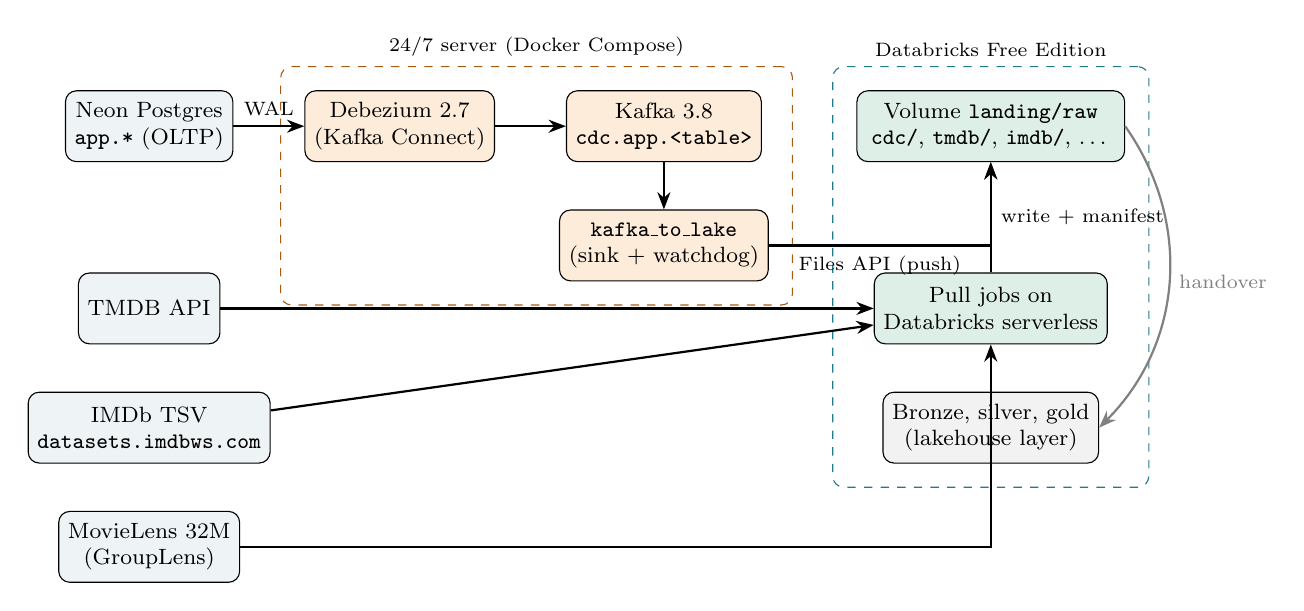
\begin{tikzpicture}[node distance=6mm and 9mm]
% sources
\node[src] (neon) {Neon Postgres\\\code{app.*} (OLTP)};
\node[src, below=14mm of neon] (tmdb) {TMDB API};
\node[src, below=of tmdb] (imdb) {IMDb TSV\\\code{datasets.imdbws.com}};
\node[src, below=of imdb] (ml) {MovieLens 32M\\(GroupLens)};
% server
\node[srv, right=of neon] (dbz) {Debezium 2.7\\(Kafka Connect)};
\node[srv, right=of dbz] (kafka) {Kafka 3.8\\\code{cdc.app.<table>}};
\node[srv, below=of kafka] (sink) {\code{kafka\_to\_lake}\\(sink + watchdog)};
% databricks
\node[dbx, right=12mm of kafka, minimum width=3.4cm] (vol) {Volume \code{landing/raw}\\\code{cdc/}, \code{tmdb/}, \code{imdb/}, \ldots};
\node[dbx, below=14mm of vol] (pull) {Pull jobs on\\Databricks serverless};
\node[box, fill=gray!10, below=of pull] (bronze) {Bronze, silver, gold\\(lakehouse layer)};

\draw[arr] (neon) -- node[above, font=\scriptsize]{WAL} (dbz);
\draw[arr] (dbz) -- (kafka);
\draw[arr] (kafka) -- (sink);
\draw[arr] (sink) -| node[pos=0.25, below, font=\scriptsize]{Files API (push)} (vol);
\draw[arr] (tmdb) -- (pull);
\draw[arr] (imdb) -- (pull);
\draw[arr] (ml) -| (pull);
\draw[arr] (pull) -- node[right, font=\scriptsize]{write + manifest} (vol);
\draw[arr, gray] (vol.east) to[bend left=40] node[right, font=\scriptsize]{handover} (bronze.east);

\begin{scope}[on background layer]
\node[draw=amberdk, dashed, rounded corners, fit=(dbz)(kafka)(sink), inner sep=3mm,
      label={[font=\scriptsize]above:24/7 server (Docker Compose)}] {};
\node[draw=teal, dashed, rounded corners, fit=(vol)(pull)(bronze), inner sep=3mm,
      label={[font=\scriptsize]above:Databricks Free Edition}] {};
\end{scope}
\end{tikzpicture}}
\caption{Two paths into the lakehouse: \emph{push} for CDC and \emph{pull} for external sources.}
\label{fig:arch}
\end{figure}

\subsection{Why CDC is pushed and APIs are pulled}
\begin{itemize}
  \item \textbf{Push for CDC}: serverless compute on Databricks Free Edition has restricted egress and cannot reach
        Kafka on the server, but the server can always call the Databricks Files API. So the sink runs on the server
        and \emph{pushes} files to the Volume (\code{ingestion/common/sinks.py}).
  \item \textbf{Pull for external sources}: serverless can reach GroupLens, TMDB and IMDb, so Databricks downloads the
        data straight to the Volume. No large file (about 1.5\,GB compressed for IMDb) has to be uploaded from a
        local machine.
\end{itemize}

\subsection{Technology stack}
\begin{table}[H]
\centering\small
\begin{tabularx}{\textwidth}{@{}lllX@{}}
\toprule
Component & Technology & Runs on & Role \\
\midrule
OLTP source & Postgres (Neon) & Cloud & App database, logical replication on \\
CDC & Debezium 2.7.3 (\code{pgoutput}) & Docker & Reads the WAL, emits every INSERT/UPDATE/DELETE \\
Message bus & Apache Kafka 3.8 (KRaft) & Docker & Topics \code{cdc.app.<table>}, 3 partitions \\
Monitoring & Kafka UI 0.7.2 & Docker & Browse topics and messages \\
Sink & Python, \code{confluent-kafka}, Databricks SDK & Docker & Kafka $\rightarrow$ JSONL on the Volume \\
Pull & Python (\code{requests}) in Databricks jobs & Serverless & Download MovieLens, IMDb; call TMDB \\
\bottomrule
\end{tabularx}
\caption{Technologies of the ingestion layer.}
\end{table}

\subsection{Why these technologies, and the alternatives considered}
\begin{longtable}{@{}p{0.17\textwidth}p{0.43\textwidth}p{0.34\textwidth}@{}}
\toprule
Technology & Why & Alternatives and why not \\
\midrule
\endhead
Debezium (log-based CDC) &
Reads the Postgres WAL, so it adds no queries to the app's database. Captures DELETEs and every intermediate version;
each change carries an LSN for ordering. No change to the app code. &
\emph{Polling} on \code{updated\_at}: misses DELETEs and UPDATEs between two polls, and loads the DB.
\emph{Triggers} into an audit table: one more write per transaction, and Neon has only 1\,GB.
\emph{Dual writes} from the app: the two targets drift apart when one side fails. \\
\addlinespace
Kafka &
Decouples source from target: Debezium keeps writing when the sink or Databricks is down. The log is kept 7 days, so
it can be replayed. Consumer-group offsets enable at-least-once delivery. More consumers (e.g.\ Flink) can be added
later without touching the source. &
Debezium Server writing straight to the target: no durable buffer; when the target is down CDC stops and Neon has to
retain WAL. \\
\addlinespace
Single-node Kafka (KRaft) &
CDC volume is only tens of MB. No ZooKeeper, which saves RAM on a small machine. &
Multi-broker cluster: more durable but too costly for the project size (see Limitations). \\
\addlinespace
Custom sink (Python) &
The Free Edition Volume is managed storage, written through the Files API. I need control over the
\emph{upload, then commit} order, the \code{dt=/hr=} layout and the Debezium watchdog. &
Ready-made sink connectors (e.g.\ S3 sink): need direct write access to object storage, which Free Edition does not
grant. \\
\addlinespace
JSONL &
One message per line, verbatim. Simple to write, readable as text by Auto Loader, no schema registry needed. &
Parquet/Avro: needs large batches and schema management inside the sink. \\
\addlinespace
\code{requests} inside Databricks jobs &
No extra infrastructure. Tokens live in a secret scope. Job-level retries. &
Download locally then upload: about 1.5\,GB of IMDb over a home connection. \\
\addlinespace
Docker Compose + Tailscale &
Rebuild everything on one machine with a few commands. Tailscale gives remote access without public ports (the
Connect REST API exposes the connector password). &
Kubernetes: too heavy for one machine. Public ports: security risk. \\
\bottomrule
\end{longtable}

\subsection{Landing-zone layout}
\begin{table}[H]
\centering\small
\begin{tabularx}{\textwidth}{@{}lX@{}}
\toprule
Folder (under \code{/Volumes/workspace/landing/raw/}) & Written by \\
\midrule
\code{cdc/<table>/dt=YYYY-MM-DD/hr=HH/part-*.jsonl} & Sink \code{kafka\_to\_lake} \\
\code{tmdb/movie\_details/dt=*/part-*.jsonl} & Job \code{tmdb\_pull} \\
\code{imdb/title\_ratings/dt=*/title.ratings.tsv.gz} & Job \code{ingest\_external} \\
\code{imdb/\{title\_basics, title\_principals, name\_basics, title\_akas\}/dt=*/} & Job \code{ingest\_external} \\
\code{movielens/ml-32m/<entity>/} & Job \code{ingest\_external} (once) \\
\code{manifests/sources/*.json} & Every pull: exact row count of each file \\
\code{state/tmdb\_pull.json} & Date of the last TMDB pull (for incremental runs) \\
\bottomrule
\end{tabularx}
\caption{Landing-zone layout.}
\end{table}

% =====================================================================
\section{Change data capture: Neon $\rightarrow$ Debezium $\rightarrow$ Kafka $\rightarrow$ Volume}
% =====================================================================

\subsection{Why log-based CDC: the polling blind spot}
Figure~\ref{fig:timeline} shows a user who rates a movie 3 stars at 10:01, changes it to 5 stars at 10:02 and
deletes it at 10:03. A job polling every 5 minutes looks at the table at 10:00 (no row yet) and 10:05 (row already
gone) and sees nothing. Debezium reads the WAL and receives all three changes, each with an increasing LSN.

\begin{figure}[H]
\centering
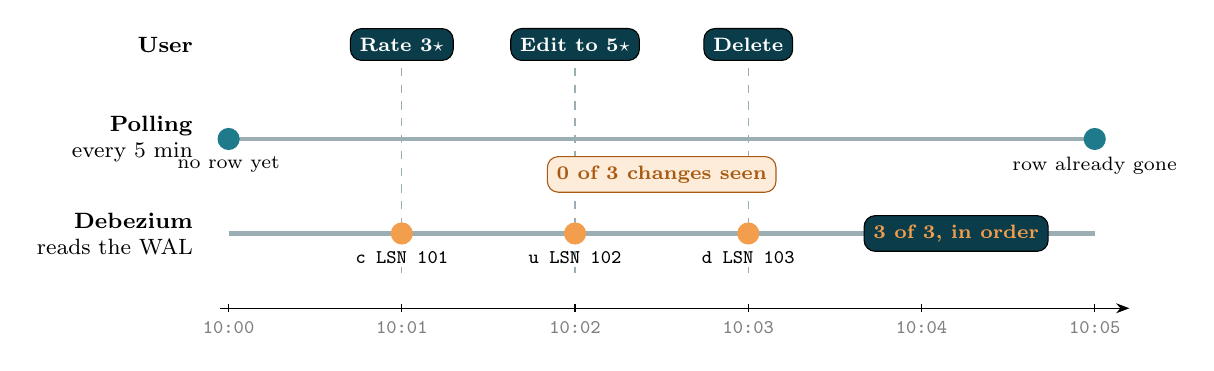
\begin{tikzpicture}[x=2.2cm, y=1cm, font=\footnotesize]
% user actions
\node[anchor=east, font=\footnotesize\bfseries] at (-0.15,2.6) {User};
\foreach \ti/\lab in {1/Rate 3$\star$, 2/Edit to 5$\star$, 3/Delete} {
  \node[draw, rounded corners, fill=dark, text=white, font=\scriptsize\bfseries] at (\ti,2.6) {\lab};
  \draw[life] (\ti,2.3) -- (\ti,-0.3);
}
% polling track
\node[anchor=east, align=right] at (-0.15,1.4) {\textbf{Polling}\\every 5 min};
\draw[greyline, line width=1.5pt] (0,1.4) -- (5,1.4);
\fill[teal] (0,1.4) circle (4pt) node[below=3pt, text=black, font=\scriptsize] {no row yet};
\fill[teal] (5,1.4) circle (4pt) node[below=3pt, text=black, font=\scriptsize] {row already gone};
\node[draw=amberdk, fill=amberlt, rounded corners, font=\scriptsize\bfseries, text=amberdk] at (2.5,0.95)
  {0 of 3 changes seen};
% WAL track
\node[anchor=east, align=right] at (-0.15,0.2) {\textbf{Debezium}\\reads the WAL};
\draw[greyline, line width=1.5pt] (0,0.2) -- (5,0.2);
\foreach \ti/\op/\lsn in {1/c/101, 2/u/102, 3/d/103}
  \fill[amber] (\ti,0.2) circle (4pt) node[below=3pt, text=black, font=\scriptsize\ttfamily] {\op{} LSN \lsn};
\node[draw, rounded corners, fill=dark, text=amber, font=\scriptsize\bfseries] at (4.2,0.2) {3 of 3, in order};
% axis
\draw[-{Stealth}] (-0.05,-0.75) -- (5.2,-0.75);
\foreach \ti in {0,...,5} {
  \draw (\ti,-0.7) -- (\ti,-0.8);
  \node[below, font=\scriptsize\ttfamily, text=gray] at (\ti,-0.8) {10:0\ti};
}
\end{tikzpicture}
\caption{Timeline: polling every 5 minutes misses all three changes; the WAL keeps them all, in order.}
\label{fig:timeline}
\end{figure}

\subsection{Captured source tables}
\begin{table}[H]
\centering\small
\begin{tabular}{@{}lll@{}}
\toprule
Table & Key & App operations \\
\midrule
\code{users} & \code{user\_id} & INSERT on sign-up \\
\code{ratings} & \code{(user\_id, movie\_id)} & UPSERT: re-rating is an UPDATE \\
\code{tags} & \code{tag\_id} & INSERT \\
\code{watchlist} & \code{(user\_id, movie\_id)} & INSERT, DELETE \\
\code{searches} & \code{search\_id} & INSERT; UPDATE of \code{clicked\_movie\_id} \\
\code{events} & \code{event\_id} & INSERT (views, playback, feedback) \\
\bottomrule
\end{tabular}
\caption{The six \code{app.*} tables under CDC.}
\end{table}

Every table uses \code{REPLICA IDENTITY FULL}, so DELETE records still carry every column (silver needs them to
check deleted rows). The \code{app\_private} schema (accounts, password hashes) is \textbf{not} in the publication.

\subsection{Debezium configuration}
The connector \code{cinelake-postgres} is declared in \code{ingestion/cdc/debezium-postgres.json}. The file holds no
secrets: the \code{\$\{CDC\_PG\_*\}} variables are filled from \code{.env} by \code{setup\_cdc.py} at registration.

\begin{lstlisting}[language=json, caption={Main Debezium connector settings}]
"plugin.name": "pgoutput",
"slot.name": "cinelake_slot",
"publication.name": "cinelake_pub",
"table.include.list": "app.users,app.ratings,app.tags,app.watchlist,app.searches,app.events",
"topic.prefix": "cdc",
"heartbeat.interval.ms": "10000",
"heartbeat.action.query": "INSERT INTO cdc_meta.heartbeat (id, ts) VALUES (1, now()) ON CONFLICT (id) DO UPDATE SET ts = EXCLUDED.ts",
"transforms": "unwrap",
"transforms.unwrap.type": "io.debezium.transforms.ExtractNewRecordState",
"transforms.unwrap.add.fields": "op,lsn,source.ts_ms",
"transforms.unwrap.delete.tombstone.handling.mode": "rewrite"
\end{lstlisting}

Design choices:
\begin{itemize}
  \item \textbf{\code{pgoutput}}: Postgres' built-in logical decoding plugin; Neon supports it without extensions.
  \item \textbf{SMT \code{ExtractNewRecordState}}: drops Debezium's \code{before/after} envelope, keeps only the new
        state and adds \code{\_\_op}, \code{\_\_lsn}, \code{\_\_source\_ts\_ms}, \code{\_\_deleted}. A DELETE becomes a
        record with \code{\_\_deleted = "true"} instead of a tombstone, so the lakehouse still sees the deletion.
  \item \textbf{Heartbeat}: every 10 seconds a row is written to \code{cdc\_meta.heartbeat}. When the app is idle the
        slot still advances, so Neon does not have to retain WAL (Neon Free is limited to 1\,GB).
  \item \textbf{JSON without embedded schema} (\code{schemas.enable=false}): small messages; the schema is managed
        downstream.
\end{itemize}

\subsection{One change, end to end}
Figure~\ref{fig:seq-cdc} follows a single re-rating through every component. The key rule is in steps 8--10: the
sink commits its Kafka offsets only after the Volume has acknowledged the file.

\begin{figure}[H]
\centering
\resizebox{\textwidth}{!}{%
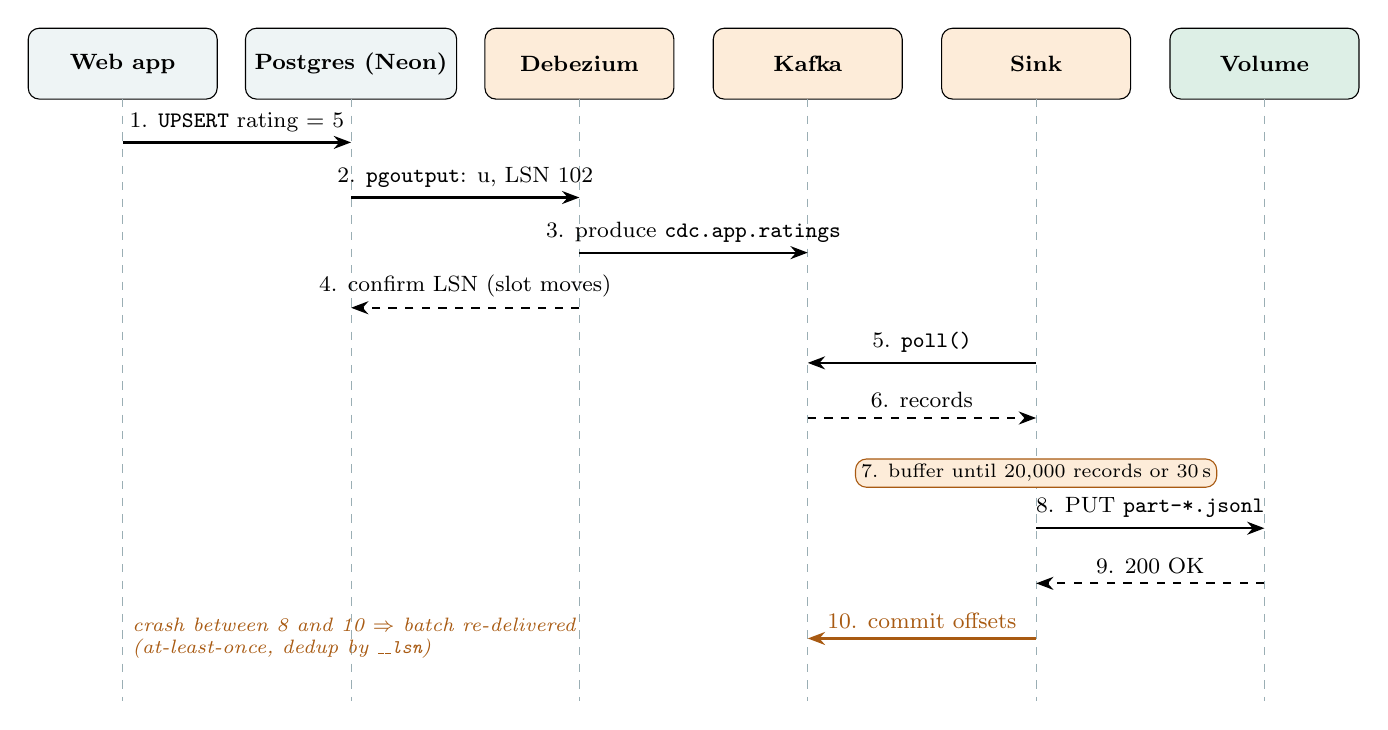
\begin{tikzpicture}[font=\footnotesize]
\def\dx{2.9}
\foreach \i/\nm/\col in {0/Web app/light, 1/Postgres (Neon)/light, 2/Debezium/amberlt, 3/Kafka/amberlt,
                      4/Sink/amberlt, 5/Volume/greenlt} {
  \node[actor=\col] at (\i*\dx,0) {\nm};
  \draw[life] (\i*\dx,-0.45) -- (\i*\dx,-8.1);
}
\draw[arr] (0,-1.0) -- node[above]{1. \code{UPSERT} rating = 5} (1*\dx,-1.0);
\draw[arr] (1*\dx,-1.7) -- node[above]{2. \code{pgoutput}: u, LSN 102} (2*\dx,-1.7);
\draw[arr] (2*\dx,-2.4) -- node[above]{3. produce \code{cdc.app.ratings}} (3*\dx,-2.4);
\draw[ret] (2*\dx,-3.1) -- node[above]{4. confirm LSN (slot moves)} (1*\dx,-3.1);
\draw[arr] (4*\dx,-3.8) -- node[above]{5. \code{poll()}} (3*\dx,-3.8);
\draw[ret] (3*\dx,-4.5) -- node[above]{6. records} (4*\dx,-4.5);
\node[self] at (4*\dx,-5.2) {7. buffer until 20,000 records or 30\,s};
\draw[arr] (4*\dx,-5.9) -- node[above]{8. PUT \code{part-*.jsonl}} (5*\dx,-5.9);
\draw[ret] (5*\dx,-6.6) -- node[above]{9. 200 OK} (4*\dx,-6.6);
\draw[arr, amberdk] (4*\dx,-7.3) -- node[above]{10. commit offsets} (3*\dx,-7.3);
\node[font=\scriptsize\itshape, text=amberdk, align=left, anchor=west] at (0,-7.3)
  {crash between 8 and 10 $\Rightarrow$ batch re-delivered\\(at-least-once, dedup by \code{\_\_lsn})};
\end{tikzpicture}}
\caption{Sequence diagram: one rating change from the web app to a JSONL file on the Volume.}
\label{fig:seq-cdc}
\end{figure}

\subsection{Least privilege}
\code{ingestion/cdc/roles.sql} creates three roles following least privilege:
\begin{itemize}
  \item \code{cinelake\_cdc} (Debezium): \code{REPLICATION}, \code{SELECT} on the 6 captured tables, and write access
        to the heartbeat row only. No rights at all on \code{app\_private}.
  \item \code{cinelake\_app} (web app and simulator) and \code{cinelake\_serving} (reverse ETL).
\end{itemize}
The roles are created in SQL by the owner, not in the Neon Console: a role created in the Console automatically
belongs to \code{neon\_superuser} and can read and write every table. In addition, \code{cinelake\_cdc} has
\code{idle\_in\_transaction\_session\_timeout = 0}. Reason: Neon kills idle transactions after 5 minutes by default,
while the initial snapshot keeps a transaction open for about 20 minutes on \code{ratings}; before the fix, Debezium
was disconnected and restarted the snapshot from scratch.

\subsection{Registering and recovering the connector}
\code{python -m ingestion.cdc.setup\_cdc} is idempotent:
\begin{itemize}
  \item default: creates the schema and write API, then registers the connector (\code{snapshot.mode = initial});
  \item \code{--roles}: also creates the least-privilege roles;
  \item \code{--status}: prints the connector and task state;
  \item \code{--snapshot-mode no\_data}: used when Kafka Connect lost its offsets but the lakehouse already has all
        data. Debezium continues from the slot position without re-snapshotting the database.
\end{itemize}
For a new database the right order is: create the schema, bulk-load the replay data, \emph{then} register the
connector. The initial snapshot \code{SELECT}s the loaded rows about 20 times faster than decoding the same rows from
the WAL, because on Neon the walsender is cut off (\code{wal\_sender\_timeout} 10\,s) while decoding large
transactions.

\subsection{Kafka}
\begin{itemize}
  \item Single-node KRaft mode (no ZooKeeper), one topic per table \code{cdc.app.<table>}, 3 partitions.
  \item The log lives on a Docker volume (\code{KAFKA\_LOG\_DIRS=/var/lib/kafka/data}), so recreating the container
        loses neither messages nor Kafka Connect offsets.
  \item 7-day retention: the long-term copy of CDC is the files on the Volume (the sink lands every change within a
        minute). Kafka only needs to cover the time the sink may be down.
  \item Ports are bound to the Tailscale IP only (\code{BIND\_ADDR}), never to a public address, because the Connect
        REST API returns the connector password.
\end{itemize}

\subsection{The \code{kafka\_to\_lake} sink}
The sink (\code{ingestion/streaming/kafka\_to\_lake.py}) is a long-running Kafka consumer (Figure~\ref{fig:flow-sink}):
\begin{enumerate}
  \item Subscribes by regex \code{\^{}cdc\textbackslash.app\textbackslash..*} and refreshes metadata every
        10 seconds to see new topics (a topic is only created on a table's first change).
  \item Buffers messages per table. Writes a file when \code{batch-size} records are buffered (default 20,000) or when
        the oldest buffered record has waited \code{flush-seconds} (default 30 seconds).
  \item Uploads each file \code{cdc/<table>/dt=/hr=/part-<time>-<uuid>.jsonl} through the Databricks Files API.
  \item \textbf{Commits offsets only after the upload} (\code{enable.auto.commit = false}).
\end{enumerate}

\begin{figure}[H]
\centering
\resizebox{\textwidth}{!}{%
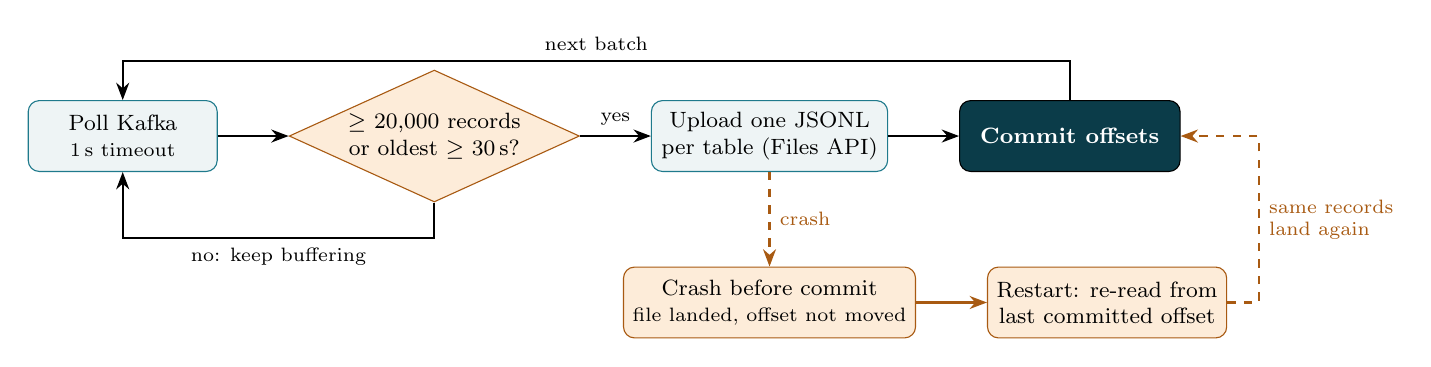
\begin{tikzpicture}[node distance=8mm and 9mm]
\node[src, draw=teal, minimum width=24mm] (poll) {Poll Kafka\\\scriptsize 1\,s timeout};
\node[dec, right=of poll] (full) {$\geq$ 20,000 records\\or oldest $\geq$ 30\,s?};
\node[src, draw=teal, right=of full, minimum width=30mm] (up) {Upload one JSONL\\per table (Files API)};
\node[box, fill=dark, text=white, right=of up, minimum width=28mm] (commit) {\textbf{Commit offsets}};
\node[box, fill=amberlt, draw=amberdk, below=12mm of up, minimum width=30mm] (crash)
  {Crash before commit\\\scriptsize file landed, offset not moved};
\node[box, fill=amberlt, draw=amberdk, right=of crash, minimum width=28mm] (restart)
  {Restart: re-read from\\last committed offset};
\draw[arr] (poll) -- (full);
\draw[arr] (full) -- node[above, font=\scriptsize]{yes} (up);
\draw[arr] (up) -- (commit);
\draw[arr] (full.south) -- ++(0,-0.45) -| node[pos=0.25, below, font=\scriptsize]{no: keep buffering} (poll.south);
\draw[arr] (commit.north) -- ++(0,0.5) -| node[pos=0.25, above, font=\scriptsize]{next batch} (poll.north);
\draw[arr, dashed, amberdk] (up) -- node[right, font=\scriptsize]{crash} (crash);
\draw[arr, amberdk] (crash) -- (restart);
\draw[arr, dashed, amberdk] (restart.east) -- ++(0.4,0) |- node[pos=0.25, right, font=\scriptsize, align=left]
  {same records\\land again} (commit.east);
\end{tikzpicture}}
\caption{Flowchart of the sink loop: land the file first, commit after.}
\label{fig:flow-sink}
\end{figure}

\begin{lstlisting}[language=Python, caption={Flush: write the files first, commit the offsets after}]
def flush(self) -> None:
    """Land every buffered table, then commit: offsets only move past data that is safely landed."""
    self.oldest = None
    if not self.pending:
        return
    now = datetime.now(timezone.utc)
    for prefix, records in self.buffers.items():
        if not records:
            continue
        relative = f"{prefix}/dt={now:%Y-%m-%d}/hr={now:%H}/part-{now:%Y%m%dT%H%M%S}-{uuid.uuid4().hex[:8]}.jsonl"
        self.sink.put(relative, b"\n".join(records) + b"\n")
        records.clear()
    self._commit()
\end{lstlisting}

\paragraph{Delivery semantics.} If the sink dies after the upload but before the commit, the batch is delivered
again: \emph{at-least-once}. Every change carries a unique \code{\_\_lsn}, and silver applies changes with a
\code{MERGE} conditioned on the LSN, so the end result is still \emph{exactly-once}. File names contain a uuid, so a
re-delivery never overwrites an earlier file.

\paragraph{A detail that matters.} The time-based flush is measured from the oldest record in the buffer, not from
the previous flush. Measured from the previous flush, an upload of 20,000 records that takes longer than
\code{flush-seconds} would cause the next record to be flushed alone, producing many one-line files.

\subsection{Watchdog that heals Debezium}
Kafka Connect does not restart a task in the \code{FAILED} state. On Neon, the task typically fails while the compute
is waking up or when the network is flaky (\code{Couldn't obtain encoding}, \code{Authentication timed out}). CDC then
stops and Neon keeps retaining WAL. Therefore, every 60 seconds the sink calls \code{restart\_failed\_tasks()}
(\code{ingestion/common/connect.py}), which reads \code{/connectors/cinelake-postgres/status} through the Connect REST
API and restarts every \code{FAILED} task, logging its \code{Caused by} line (Figure~\ref{fig:seq-watchdog}).

\begin{figure}[H]
\centering
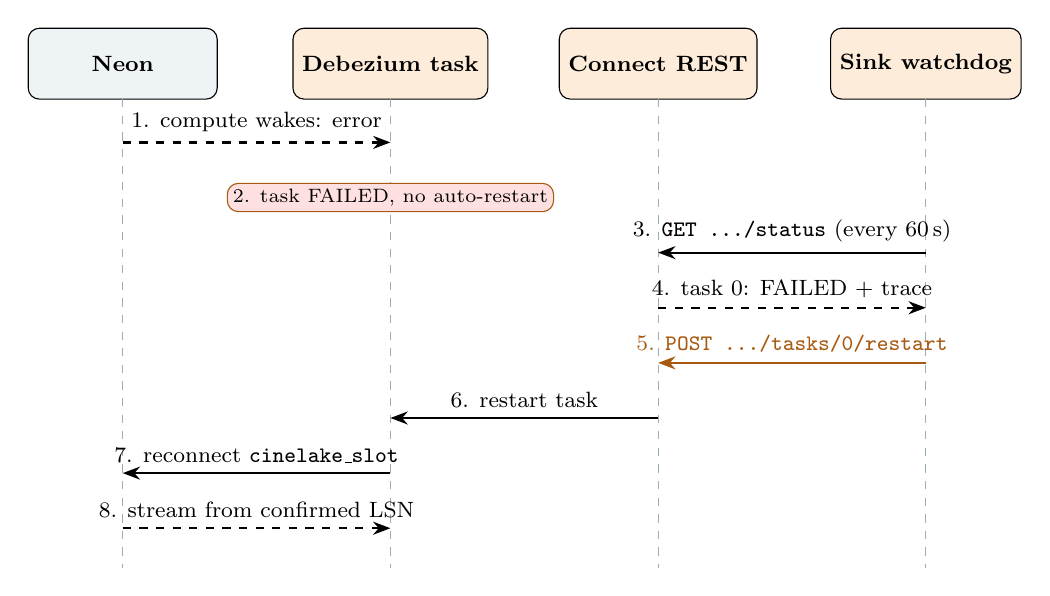
\begin{tikzpicture}[font=\footnotesize]
\def\dx{3.4}
\foreach \i/\nm/\col in {0/Neon/light, 1/Debezium task/amberlt, 2/Connect REST/amberlt, 3/Sink watchdog/amberlt} {
  \node[actor=\col] at (\i*\dx,0) {\nm};
  \draw[life] (\i*\dx,-0.45) -- (\i*\dx,-6.4);
}
\draw[ret] (0,-1.0) -- node[above]{1. compute wakes: error} (1*\dx,-1.0);
\node[self, fill=red!12] at (1*\dx,-1.7) {2. task FAILED, no auto-restart};
\draw[arr] (3*\dx,-2.4) -- node[above]{3. \code{GET .../status} (every 60\,s)} (2*\dx,-2.4);
\draw[ret] (2*\dx,-3.1) -- node[above]{4. task 0: FAILED + trace} (3*\dx,-3.1);
\draw[arr, amberdk] (3*\dx,-3.8) -- node[above]{5. \code{POST .../tasks/0/restart}} (2*\dx,-3.8);
\draw[arr] (2*\dx,-4.5) -- node[above]{6. restart task} (1*\dx,-4.5);
\draw[arr] (1*\dx,-5.2) -- node[above]{7. reconnect \code{cinelake\_slot}} (0,-5.2);
\draw[ret] (0,-5.9) -- node[above]{8. stream from confirmed LSN} (1*\dx,-5.9);
\end{tikzpicture}
\caption{Sequence diagram: the watchdog restarts a failed Debezium task; no change is lost because the slot keeps
the confirmed LSN.}
\label{fig:seq-watchdog}
\end{figure}

% =====================================================================
\section{External APIs: pull ingestion on Databricks}
% =====================================================================

\subsection{Common principles}
\begin{itemize}
  \item \textbf{Raw-first}: keep the source data as is (original TSV/CSV files, verbatim JSON responses). Silver can be
        rebuilt at any time without calling the source again.
  \item \textbf{Idempotent}: if the manifest of a pull exists, the pull is skipped, unless the widget
        \code{force=true} is set.
  \item \textbf{Manifest}: each pull writes \code{manifests/sources/<name>.json} with the exact row count of every
        file. Reconciliation check R1 on Databricks compares these counts with bronze.
  \item \textbf{Retries}: the \code{ingest\_external} and \code{tmdb\_pull} tasks retry once after 60 seconds on
        transient network errors.
\end{itemize}

\subsection{IMDb}
Notebook \code{02\_ingest\_external.py}, code \code{src/movie\_lakehouse/ingest/external.py}.

\begin{figure}[H]
\centering
\begin{minipage}[c]{0.56\textwidth}
\centering
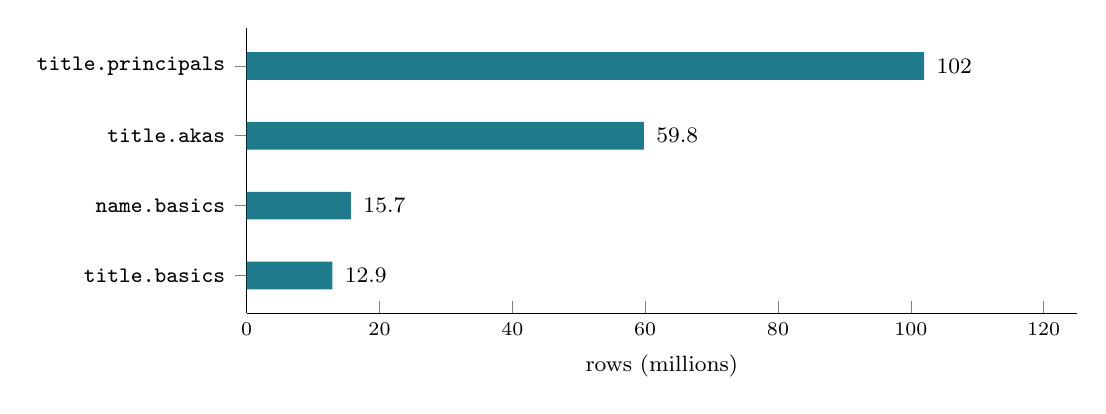
\begin{tikzpicture}
\begin{axis}[
  xbar, width=\textwidth, height=5.2cm,
  xmin=0, xmax=125,
  symbolic y coords={title.basics, name.basics, title.akas, title.principals},
  ytick=data, yticklabel style={font=\footnotesize\ttfamily},
  xlabel={rows (millions)}, xlabel style={font=\footnotesize},
  xticklabel style={font=\scriptsize},
  point meta=x, nodes near coords, nodes near coords style={font=\footnotesize\bfseries},
  every node near coord/.append style={xshift=1pt},
  bar width=10pt, enlarge y limits=0.18,
  axis x line*=bottom, axis y line*=left]
\addplot[fill=teal, draw=none] coordinates
  {(12.9,title.basics) (15.7,name.basics) (59.8,title.akas) (102,title.principals)};
\end{axis}
\end{tikzpicture}
\end{minipage}\hfill
\begin{minipage}[c]{0.4\textwidth}
\centering
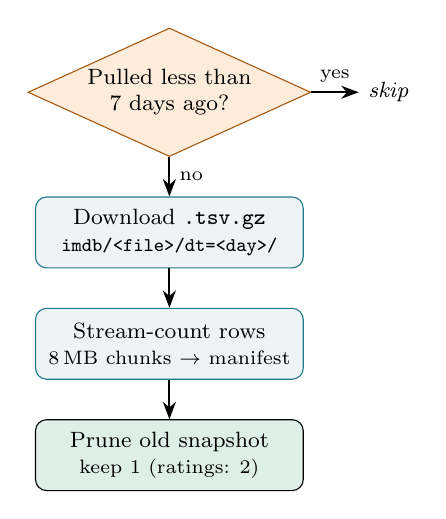
\begin{tikzpicture}[node distance=5mm]
\node[dec] (age) {Pulled less than\\7 days ago?};
\node[src, draw=teal, below=of age, minimum width=34mm] (dl) {Download \code{.tsv.gz}\\\scriptsize\code{imdb/<file>/dt=<day>/}};
\node[src, draw=teal, below=of dl, minimum width=34mm] (cnt) {Stream-count rows\\\scriptsize 8\,MB chunks $\rightarrow$ manifest};
\node[dbx, below=of cnt, minimum width=34mm] (pr) {Prune old snapshot\\\scriptsize keep 1 (ratings: 2)};
\node[right=6mm of age, font=\footnotesize\itshape] (skip) {skip};
\draw[arr] (age) -- node[above, font=\scriptsize]{yes} (skip);
\draw[arr] (age) -- node[right, font=\scriptsize]{no} (dl);
\draw[arr] (dl) -- (cnt);
\draw[arr] (cnt) -- (pr);
\end{tikzpicture}
\end{minipage}
\caption{IMDb: rows per downloaded file (about 190 million in total), and the weekly pull flow.}
\label{fig:imdb}
\end{figure}

\begin{table}[H]
\centering\small
\begin{tabularx}{\textwidth}{@{}llXr@{}}
\toprule
Bronze table & IMDb file & Used for & Rows \\
\midrule
\code{imdb\_ratings} & \code{title.ratings} & Score and vote count & -- \\
\code{imdb\_titles} & \code{title.basics} & Title type, runtime & 12.9 M \\
\code{imdb\_principals} & \code{title.principals} & Directors, cast & 102 M \\
\code{imdb\_names} & \code{name.basics} & Names, professions & 15.7 M \\
\code{imdb\_akas} & \code{title.akas} & Localized titles (e.g.\ Vietnamese) & 59.8 M \\
\bottomrule
\end{tabularx}
\caption{IMDb files downloaded (about 1.5\,GB compressed).}
\end{table}

\begin{itemize}
  \item IMDb publishes \emph{full snapshots} with no incremental API. Each source is therefore downloaded at most once
        every 7 days (\code{IMDB\_MIN\_DAYS\_BETWEEN\_PULLS}) into \code{imdb/<file>/dt=<day>/}.
  \item Rows are counted by streaming the decompressed data in 8\,MB chunks, without extracting to disk (the
        uncompressed files are several GB).
  \item \textbf{Bounded snapshots}: \code{title.ratings} keeps 2 snapshots, the four large files keep 1. The function
        \code{prune\_imdb\_snapshots} removes the old snapshot's bronze rows, landing folder and manifest together, so
        reconciliation between bronze and manifests still matches.
  \item \code{title.crew} (duplicates \code{principals}) and \code{title.episode} (TV episodes) are not downloaded.
\end{itemize}

\subsection{TMDB API}
Notebook \code{05\_tmdb\_pull.py}, code \code{src/movie\_lakehouse/ingest/tmdb.py}.

\paragraph{Which movies.} Every \code{tmdb\_id} linked to a MovieLens movie (through \code{links.csv}) that at least one
sampled user has rated. Each movie is fetched with \code{/movie/\{id\}?append\_to\_response=videos,keywords} (details,
trailers and keywords in one request).

\paragraph{Fault-tolerant client.}
\begin{itemize}
  \item 16 threads (\code{ThreadPoolExecutor}) share one \code{RateLimiter} (at most 35 requests/second, below TMDB's
        limit).
  \item On network errors, HTTP 429 or 5xx: up to 6 retries, honouring the \code{Retry-After} header, otherwise a
        $2^{n}$-second backoff. When retries run out, status \code{599} is recorded so the next run tries again.
  \item The token lives in the Databricks secret scope \code{cinelake/tmdb\_token}, never in code or \code{.env}.
        The client accepts both the Read Access Token (Bearer) and the v3 API key.
\end{itemize}

\paragraph{Incremental.} Figure~\ref{fig:flow-tmdb} shows how each ID is handled.
\begin{enumerate}
  \item IDs that already have a final result (\code{200} or \code{404}) are skipped. Other statuses are retried.
  \item From the second run on, \code{state/tmdb\_pull.json} gives the date of the previous pull, and
        \code{/movie/changes} is queried (at most 14 days per query, paginated). Any changed ID that belongs to the
        catalog is fetched again.
  \item A JSONL file is written every 2,000 responses, so an interrupted job keeps what it already fetched.
\end{enumerate}

\begin{figure}[H]
\centering
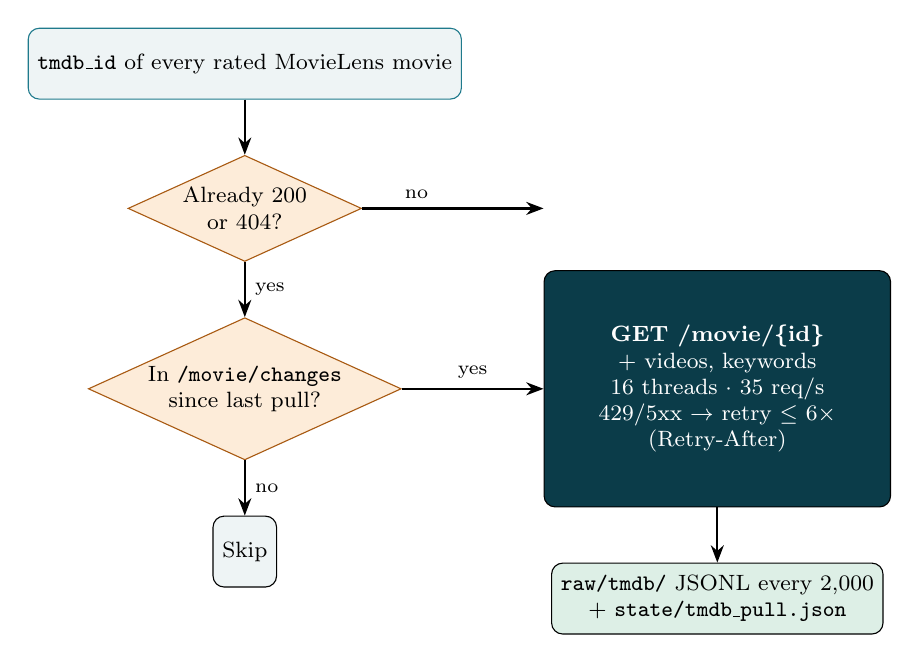
\begin{tikzpicture}[node distance=7mm and 10mm]
\node[src, draw=teal] (ids) {\code{tmdb\_id} of every rated MovieLens movie};
\node[dec, below=of ids] (final) {Already 200\\or 404?};
\node[dec, below=of final] (chg) {In \code{/movie/changes}\\since last pull?};
\node[src, below=of chg] (skip) {Skip};
\node[box, fill=dark, text=white, right=18mm of chg, minimum width=44mm, minimum height=30mm] (get)
  {\textbf{GET /movie/\{id\}}\\+ videos, keywords\\16 threads $\cdot$ 35 req/s\\429/5xx $\rightarrow$ retry $\leq$ 6$\times$\\(Retry-After)};
\node[dbx, below=of get] (out) {\code{raw/tmdb/} JSONL every 2,000\\+ \code{state/tmdb\_pull.json}};
\draw[arr] (ids) -- (final);
\draw[arr] (final) -- node[right, font=\scriptsize]{yes} (chg);
\draw[arr] (chg) -- node[right, font=\scriptsize]{no} (skip);
\draw[arr] (final.east) -- node[above, font=\scriptsize, pos=0.3]{no} (final.east -| get.west);
\draw[arr] (chg) -- node[above, font=\scriptsize]{yes} (get);
\draw[arr] (get) -- (out);
\end{tikzpicture}
\caption{Flowchart: which TMDB movies are fetched on each run.}
\label{fig:flow-tmdb}
\end{figure}

\begin{lstlisting}[language=json, caption={One TMDB record on the landing zone (raw-first)}]
{"tmdb_id": "603", "fetched_at": "2026-10-18T02:11:05+00:00",
 "http_status": "200", "raw_json": "{\"id\": 603, \"title\": \"The Matrix\", ...}"}
\end{lstlisting}

\paragraph{Effect.} The first pull needed about 45 thousand requests and took 23 minutes. Later runs need only 211
requests (new IDs and IDs listed by \code{/changes}) and take 17 seconds (Figure~\ref{fig:tmdb-chart}).

\begin{figure}[H]
\centering
\begin{tikzpicture}
\begin{groupplot}[
  group style={group size=2 by 1, horizontal sep=2.2cm},
  ybar, width=6.5cm, height=5.5cm, ymode=log, log origin=infty,
  symbolic x coords={First pull, Incremental}, xtick=data,
  enlarge x limits=0.5, bar width=22pt,
  nodes near coords, nodes near coords style={font=\footnotesize\bfseries},
  point meta=rawy,
  every node near coord/.append style={/pgf/number format/fixed, /pgf/number format/1000 sep={,}},
  ticklabel style={font=\scriptsize}, title style={font=\small\bfseries},
  axis x line*=bottom, axis y line*=left]
\nextgroupplot[title={Requests (log scale)}, ymin=10, ymax=300000]
\addplot[fill=teal, draw=none] coordinates {(First pull,45000) (Incremental,211)};
\nextgroupplot[title={Wall time, seconds (log scale)}, ymin=1, ymax=10000]
\addplot[fill=amber, draw=none] coordinates {(First pull,1380) (Incremental,17)};
\end{groupplot}
\end{tikzpicture}
\caption{TMDB first pull vs.\ incremental run: about 200 times fewer requests, 80 times faster.}
\label{fig:tmdb-chart}
\end{figure}

\subsection{MovieLens 32M}
The zip file is downloaded once and extracted into 4 entities (\code{movies}, \code{ratings}, \code{tags},
\code{links}), each with a row-count manifest (header excluded). Since the manifest exists, later runs skip it.

% =====================================================================
\section{Demo}
% =====================================================================

The demo follows the three numbered paths of Figure~\ref{fig:kafka-arch}: \textcircled{\scriptsize 1} a rating in
the web app reaches Kafka within seconds, \textcircled{\scriptsize 2} the sink pushes it to Databricks as a JSONL
file, and \textcircled{\scriptsize 3} the external sources are pulled by Databricks.

\begin{figure}[H]
\centering
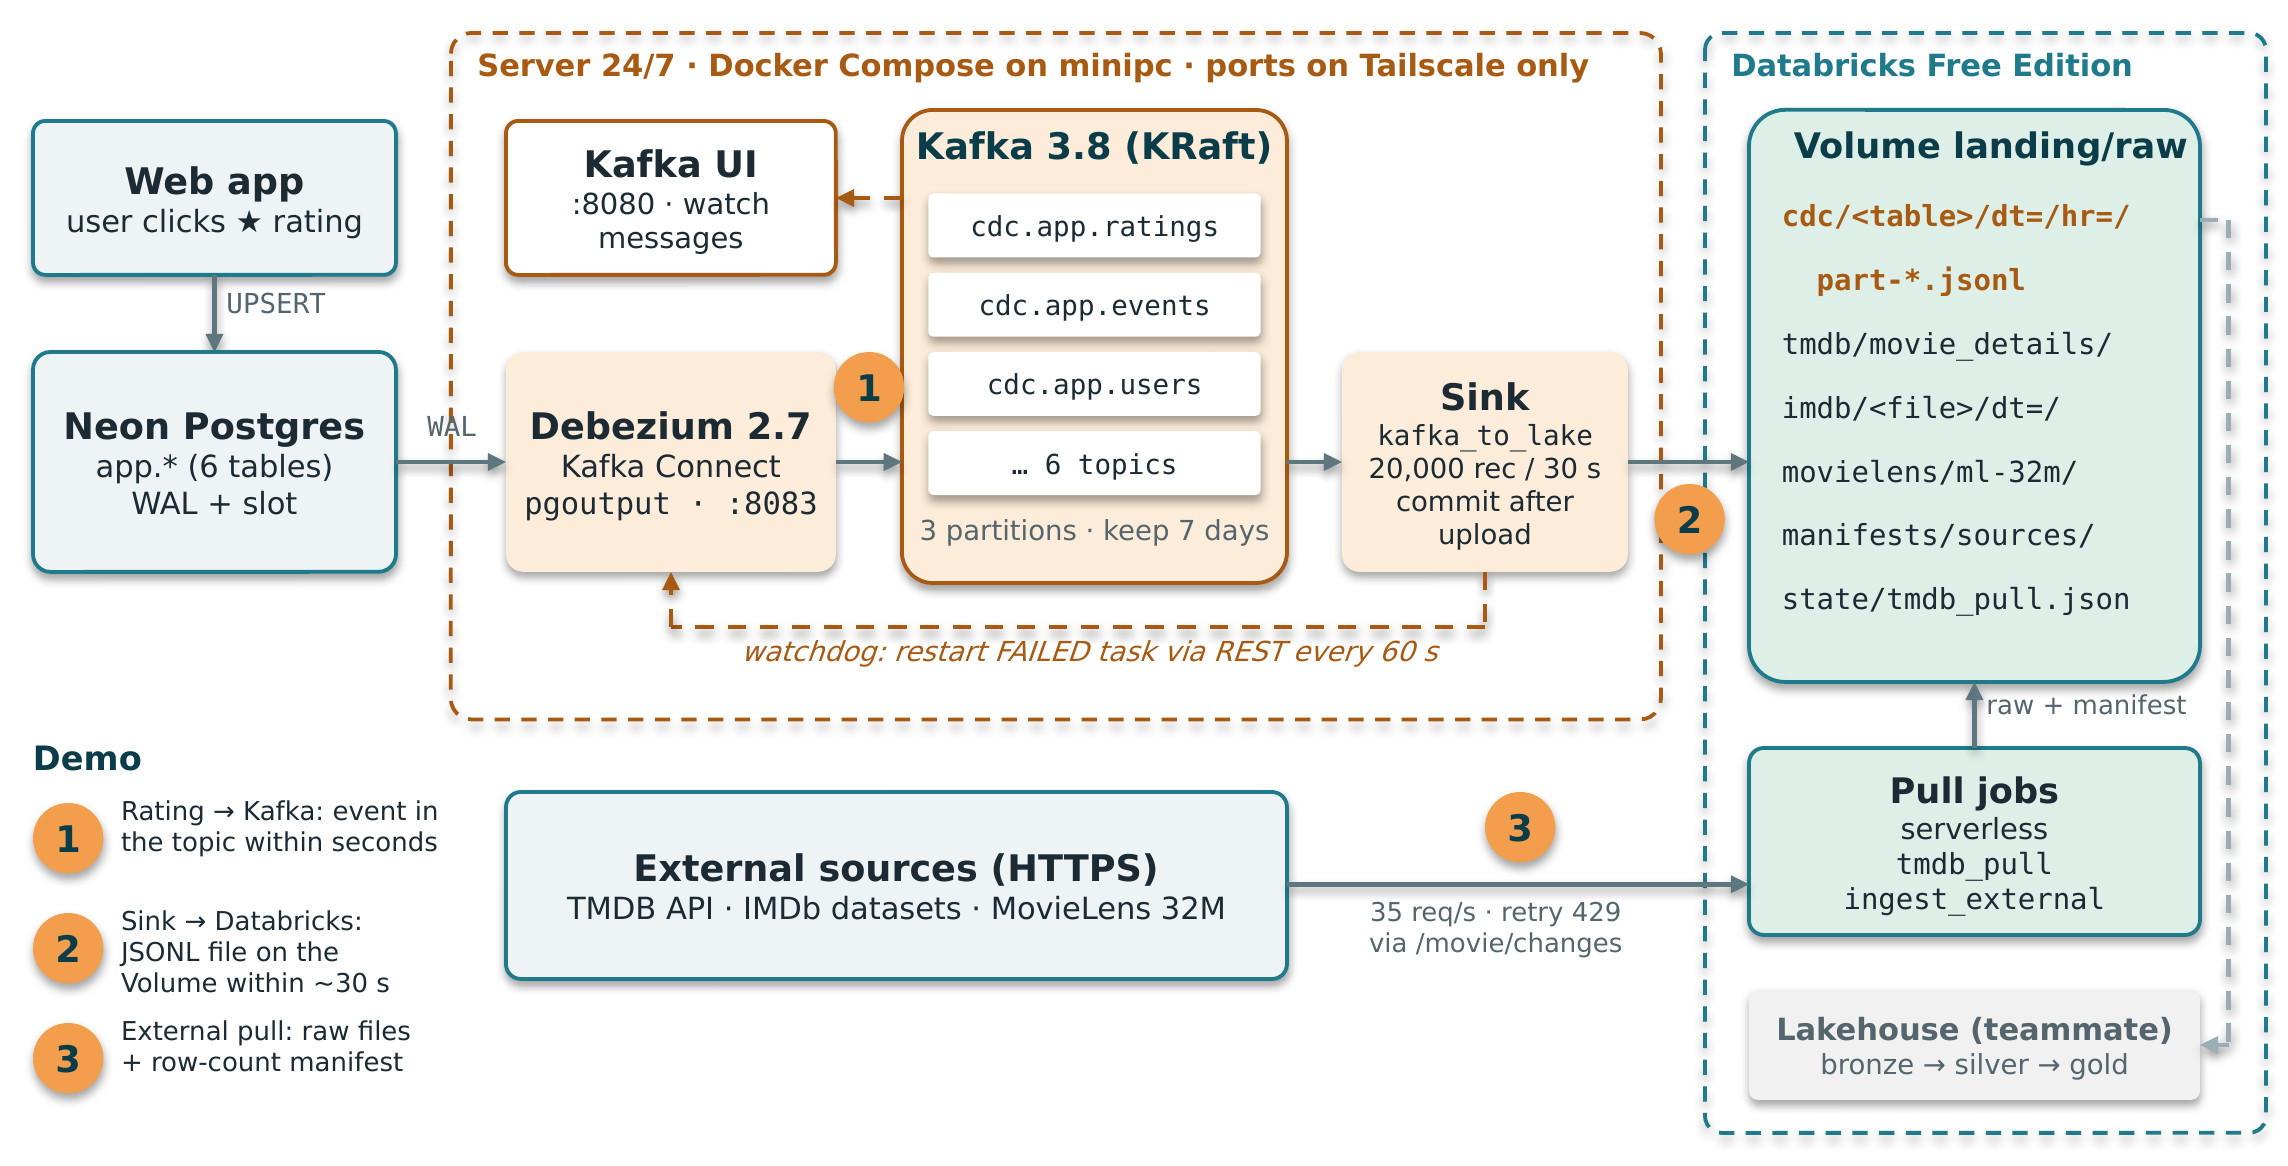
\includegraphics[width=0.9\textwidth]{figures/kafka-architecture.png}
\caption{Ingestion architecture around Kafka, with the three demo paths numbered.}
\label{fig:kafka-arch}
\end{figure}

\paragraph{Before the demo.} On the server, every service must be up and the connector running:
\begin{lstlisting}[language=bash, caption={Pre-demo checks on the server}]
docker compose ps                                  # kafka, connect, kafka-ui, sink: Up
.venv/bin/python -m ingestion.cdc.setup_cdc --status   # connector + task 0: RUNNING
docker compose logs -f sink                        # keep this open for demo 2
\end{lstlisting}

\subsection{Demo 1: a rating reaches Kafka within seconds}
\textbf{Goal}: show that a change in the app database is captured from the WAL and appears in Kafka almost
immediately, with no polling.
\begin{enumerate}
  \item Open Kafka UI (\code{http://<tailscale-ip>:8080}) $\rightarrow$ \emph{Topics} $\rightarrow$
        \code{cdc.app.ratings} $\rightarrow$ \emph{Messages}, sorted newest first.
  \item In the web app, rate a movie (or change an existing rating).
  \item Refresh Kafka UI: a new message appears. Point out \code{\_\_op} (\code{c} for a first rating, \code{u} for a
        re-rating), \code{\_\_lsn} and \code{\_\_source\_ts\_ms}.
  \item Compare \code{\_\_source\_ts\_ms} (commit time in Postgres) with the Kafka message timestamp shown by Kafka UI:
        the gap is in the order of milliseconds to a few seconds.
\end{enumerate}
\begin{lstlisting}[language=json, caption={A rating message as seen in Kafka UI and later in the JSONL file}]
{"user_id":185042,"movie_id":12429,"rating":"3.0","rated_at":"2026-11-07T16:48:49Z","source":"app",
 "created_at":"2026-11-07T18:03:00Z","updated_at":"2026-11-07T18:03:00Z",
 "__deleted":"false","__op":"c","__lsn":2274258168,"__source_ts_ms":1794074581487}
\end{lstlisting}
\textbf{What it proves}: log-based CDC catches every change as it is committed. Even when the app is idle, the
10-second heartbeat keeps the slot moving, so the next real change is not delayed by retained WAL.

\screenshot{figures/demo1-kafka-ui.png}{Demo 1: the new rating message in topic \code{cdc.app.ratings} (Kafka UI).}{fig:demo1}

\subsection{Demo 2: the sink pushes JSONL to Databricks}
\textbf{Goal}: show the micro-batch landing on the Volume, and that offsets are committed only after the upload.
\begin{enumerate}
  \item Watch the sink log. Within at most \code{flush-seconds} (30\,s) after the rating, a line appears:
\begin{lstlisting}[language=bash, numbers=none]
[sink] 1 records -> cdc/ratings/dt=2026-11-08/hr=15/part-20261108T152301-3f9c2a1b.jsonl (total ... in ... files)
\end{lstlisting}
  \item In Databricks, open \emph{Catalog} $\rightarrow$ \code{workspace.landing.raw} $\rightarrow$
        \code{cdc/ratings/dt=<today>/hr=<hour>/} and open the new file: one JSON line per change, identical to the
        Kafka message of demo 1.
  \item Optionally, query it directly from a notebook:
\begin{lstlisting}[language=SQL, numbers=none]
SELECT user_id, movie_id, rating, __op, __lsn, __source_ts_ms
FROM json.`/Volumes/workspace/landing/raw/cdc/ratings/dt=2026-11-08/`
ORDER BY __lsn DESC LIMIT 5;
\end{lstlisting}
  \item Optionally, \code{.venv/bin/python -m ingestion.trace --last 5} prints the timestamps of the change at every
        hop (commit, file on the Volume, and the lakehouse hops once the teammate's jobs have run).
\end{enumerate}
\textbf{What it proves}: the change lands as JSONL in under a minute; the file name contains a uuid, and offsets move
only after the file exists (Figure~\ref{fig:seq-cdc}, steps 8--10).

\screenshot{figures/demo2-volume-jsonl.png}{Demo 2: the sink log line and the JSONL file on the Volume.}{fig:demo2}

\subsection{Demo 3: pulling external sources}
\textbf{Goal}: show the pull path and its incremental behaviour.
\begin{enumerate}
  \item In the Databricks workspace, open notebook \code{05\_tmdb\_pull.py} and run it (widget \code{limit} can be set
        to a small number such as 200 for a short demo). The last cell prints the manifest of the run: number of
        requests, statuses and files written.
  \item Run it a second time: thanks to the skip rule and \code{/movie/changes}, it only fetches new or changed IDs
        (in production: 211 requests and 17 seconds instead of 45,000 and 23 minutes).
  \item Open notebook \code{02\_ingest\_external.py} and run it with \code{force=false}: IMDb and MovieLens are skipped
        because their manifests exist and the last IMDb pull is less than 7 days old.
  \item Show the result in \emph{Catalog}: \code{raw/tmdb/movie\_details/dt=<today>/part-*.jsonl},
        \code{state/tmdb\_pull.json}, and a manifest in \code{manifests/sources/} with its row counts.
\end{enumerate}
\textbf{What it proves}: external sources are stored raw, the pull is idempotent and incremental, and every pull leaves
a manifest that the lakehouse layer can reconcile against.

\screenshot{figures/demo3-tmdb-pull.png}{Demo 3: output of \code{tmdb\_pull} and the files and manifest it wrote.}{fig:demo3}

% =====================================================================
\section{Operations and handover}
% =====================================================================

\subsection{Handover to the lakehouse layer}
The ingestion layer ends at the landing zone. The lakehouse layer (bronze, silver, gold) is owned by a teammate and
reads files from \code{/Volumes/workspace/landing/raw/}. Both sides agree on a data contract (details in the handover
file \code{HANDOVER\_INGESTION\_TO\_LAKEHOUSE.md}):
\begin{itemize}
  \item \textbf{CDC}: each JSONL line is one change, with the table's columns (strings or numbers) plus
        \code{\_\_op} (\code{r}, \code{c}, \code{u}, \code{d}), \code{\_\_lsn}, \code{\_\_source\_ts\_ms}, \code{\_\_deleted}.
  \item \textbf{At-least-once delivery}: a change may appear more than once; the lakehouse dedups and orders by
        \code{\_\_lsn}.
  \item \textbf{Batch sources}: raw files plus a row-count manifest in \code{manifests/sources/} for reconciliation.
\end{itemize}

\subsection{Running 24/7}
The whole CDC part runs with Docker Compose (project \code{movie-lakehouse}) on \code{minipc}:
\begin{lstlisting}[language=bash, caption={Setup on the server}]
python3 -m venv .venv && .venv/bin/pip install -e ".[ingestion]"
docker compose up -d kafka connect kafka-ui
.venv/bin/python -m ingestion.cdc.setup_cdc --snapshot-mode no_data
docker compose --profile server up -d --build sink
\end{lstlisting}
\begin{itemize}
  \item Every service has \code{restart: unless-stopped}. Heap sizes are capped (Kafka 512\,MB, Connect 768\,MB) so the
        small machine keeps RAM for the sink and the daily jobs.
  \item New CDC files on the Volume fire the file-arrival trigger of job \code{cinelake\_refresh}
        (60 seconds after the last file, at least 6 hours between runs because of the Free Edition quota).
  \item A cron job at 01:00 runs \code{ingestion/simulator/run.py} (simulated behaviour through the app's own API, so
        it also flows through CDC), then \code{ingestion/retention.py}.
\end{itemize}

\subsection{Retention on Neon}
Neon Free has only 1\,GB, while \code{app.events} is an append-only log that keeps growing. \code{retention.py}
deletes events older than \code{RETENTION\_DAYS} (60 days) in batches of 50,000 rows so transactions stay short and
the WAL is streamed gradually, then runs \code{VACUUM}. The lakehouse still keeps the full history: in WAL order, an
event's INSERT always precedes its DELETE, and silver does not apply DELETEs of \code{app.events}.

\subsection{Checks and troubleshooting}
\begin{table}[H]
\centering\small
\begin{tabularx}{\textwidth}{@{}lXX@{}}
\toprule
Check & Command / where & Passes when \\
\midrule
Debezium & \code{python -m ingestion.cdc.setup\_cdc --status} & Connector and task \code{RUNNING} \\
Kafka & Kafka UI, topics \code{cdc.app.*} & New messages after each action in the app \\
Sink & \code{docker compose logs -f sink} & Line \code{[sink] N records -> cdc/<table>/...} \\
Volume & Catalog \code{workspace.landing.raw/cdc/} & New files every hour \\
End-to-end & \code{python -m ingestion.trace --last 5} & Every hop has a time, up to \code{serving.*} \\
\bottomrule
\end{tabularx}
\caption{Operations checklist.}
\end{table}

\begin{table}[H]
\centering\small
\begin{tabularx}{\textwidth}{@{}XX@{}}
\toprule
Symptom & Fix \\
\midrule
Debezium task \code{FAILED} & The watchdog restarts it every minute. If it keeps failing, check the \code{connect}
log and the network to Neon \\
Sink cannot log in to Databricks & Token expired: update \code{DATABRICKS\_TOKEN}, restart \code{sink} \\
Neon slot retains a lot of WAL & Connect has been down for long: start it. After several days, re-register with
\code{--snapshot-mode no\_data} \\
Two Debezium connectors on one slot & Only one connector may read \code{cinelake\_slot}: stop the old one before
registering a new one \\
\bottomrule
\end{tabularx}
\caption{Common incidents.}
\end{table}

% =====================================================================
\section{Evaluation}
% =====================================================================

\subsection{Data correctness}
\begin{itemize}
  \item \textbf{Manifest (R1)}: every batch file has an exact row count, so the lakehouse can reconcile after loading.
  \item \textbf{CDC reconciliation (R2)}: the number of rows replayed into Neon must equal the number of rows received
        through CDC (e.g.\ 597,897 = 597,897).
  \item \textbf{No loss, no duplicates}: offsets are committed only after the upload, combined with MERGE by LSN in
        silver.
\end{itemize}

\subsection{Latency}
\begin{table}[H]
\centering\small
\begin{tabularx}{\textwidth}{@{}lXl@{}}
\toprule
Segment & Nature & Latency \\
\midrule
Postgres $\rightarrow$ Debezium $\rightarrow$ Kafka & True streaming, change by change & Milliseconds to seconds \\
Kafka $\rightarrow$ Volume & Sink micro-batch (flush by size or time) & Under 1 minute \\
Volume $\rightarrow$ serving (lakehouse layer) & \code{availableNow} job on new files & About 12 minutes \\
\bottomrule
\end{tabularx}
\caption{Latency per segment (measured on the End-to-end trace page, 18/10/2026: 11.9 minutes from commit to serving).}
\end{table}

CDC latency is computed in silver as \code{\_ingested\_at} $-$ \code{\_source\_ts}. The \code{ingestion.trace} command
prints the time of one LSN at every hop and serves as evidence for the end-to-end demo.

\subsection{Pull efficiency}
\begin{itemize}
  \item TMDB incremental: from about 45,000 requests (23 minutes) on the first run down to 211 requests (17 seconds)
        on later runs (Figure~\ref{fig:tmdb-chart}).
  \item IMDb: at most once a week. Only 1 snapshot is kept for the four large files (about 190 million rows), so
        storage does not grow over time (Figure~\ref{fig:imdb}).
\end{itemize}

% =====================================================================
\section{Conclusion}
% =====================================================================

\paragraph{Results.} The ingestion layer brings all four kinds of sources (CSV, TSV, JSON API, CDC) into the lakehouse
under one principle: keep data raw, traceable and reconcilable. CDC runs 24/7 on the server: files are written before
offsets are committed (at-least-once, combined with the LSN for exactly-once), with a self-healing watchdog and least
privilege. API pulls tolerate network errors and rate limits, and are incremental and idempotent.

\paragraph{Limitations.}
\begin{itemize}
  \item One Kafka broker, replication factor 1: no tolerance to a hardware failure of the server (the Volume remains
        the long-term copy).
  \item Commit-to-serving latency of about 12 minutes, bounded by the Databricks Free Edition compute quota, not by CDC.
  \item IMDb has no incremental API, so each pull downloads a full snapshot again.
\end{itemize}

\paragraph{Future work.}
\begin{itemize}
  \item Multi-broker Kafka and a Schema Registry (Avro) to manage schema changes.
  \item A stream processor (Flink or continuous Structured Streaming) reading Kafka directly to refresh signals within
        seconds.
  \item More sources (OMDb, Trakt) following the same pattern: rate-limited client, raw storage, manifest.
\end{itemize}

\end{document}
